\chapter{Hidden Markov Model design}

%This is what I did to test and confirm my hypothesis.


%You may want to split this chapter into sub chapters depending on your design. I suggest you change
%the title to something more specific to your project.

%This is where you describe your design process in detail, from component/device selection to actual
%design implementation, to how you tested your system. Remember detail is important in technical
%writing. Do not just write I used a computer give the computer specifications or the oscilloscopes part
%number. Describe the system in enough detail so that someone else can replicate your design as well
%as your testing methodology.

%If you use or design code for your system, represent it as flow diagrams in text.

This section focuses on the design of the HMM used to test the hyphotheses postulated above.

\section{Description of available dataset}

The available dataset was acquired from a moving dog using Inertia Measurement Units. 
Two inertial measurements units (IMU) were straped to the front and back of a dog. Each unit has an accelarometer, a gyroscope and a magnetometer. The dataset contains calibrated measurements of a dog running, walking, or trotting then walking; together with the footfalls. The footfall is a binary value that indicates the state of the dog's leg: if it is on or above the ground, at a particular instant in its gait sequence. 
The four variables representing the footfalls effectively constitutes the ground truth informing us about the state in which the dog is at any time of the gait sequence.

The dataset can be retrieved from nine different matlab files. Each file contains twenty four matlab variables. The variables of interest are listed below. 

\begin{center} \label{dataset}
	\begin{tabular}{ |c|c|c|c| } 
		\hline
		\multicolumn{2}{| c |}{Observations} {Footfalls}\\
		\hline
		& Accelerometer & Gyroscope & Magnetometer \\ 
		 \hline
 


	  	Front & accFrontX & FrontPitch & magFront\_cal\\
		 	  & accFrontY & FrontRoll & magFront\_cal2\\
		      & accFrontZ & FrontYaw & magFront\_cal3\\
		      \hline
		 
		Back  & accBackX & BackPitch & magBack\_cal\\
		      & accBackY & BackRoll & magBack\_cal2\\
		      & accBackZ & BackYaw & magBack\_cal3\\
    \hline

	\end{tabular}
\end{center}

The observations are continous and the statistical property are assumed to be stationary, i.e, the do not vary over time. In this sta
\subsubsection{stationary: statistical property do not vary over time or non-stationary: properties vary over time}

\subsubsection{pure or corrupted?}

\subsection{Gait sequence modelling}
One of the objectives of this project is to effectively model the gait sequence dynamic of the dog using IMU measurements.
The gait sequence was modelled as a succession of hidden or latent states observed by the IMU measurements.

\subsubsection{States and observation }
The state space is 
\begin{align} \label{eq:state}
S &= {S_i} = \{(LF, RF, LB, RB)\} = \{0000, 0001, 0010, ..., 1111\}. \\
i &= 1, 2, ..., 16
\end{align}
is made up of 16 different states that steam from the combination of the four binary footfalls as shown in equation. \ref{eq:state}

The states sequences are observed through the IMU measurements that form the feature space. An observation instance is a row vector of K dimensions. The initial K value is 18 from the 18 IMU measurements.
Thus the observation sequence O is an TxK matrix of continuous values as presented in \ref{eq:obs}. T is the number of observations in a sequence.
\begin{align} \label{eq:obs}
O &= \{Ok_t\} = O1_t, O2_t, ..., O18_t. \\
k &= 1, 2, ..., 18. \\
t &= 1, 2, ..., T.
\end{align}


\subsubsection{Splitting the design into front and back module}
To reduce the HMM model's complexity, it was broken down into front and back sub-HMM. These two models may be combined to get back the holistic 16-states model.
This simplifies the model by reducing the number of states from 16 down to 4 states. 
This design design was motivated by the fact that it is a simpler task to classify 4 classses than discriminating between 16 classes. The remainig of this section will focus on the design of the 4-states HMM model.
 
\subsubsection{Transition between states}
%%TODO: fix the subscript
This design assumes that a dog can transition from one state to any other possible state. So, for any transtion from S\_{i} to S\_{j} both S\_{i} and S\_{j} may be any of the element of the state space 

\[S = \{S1, S2, S3, S4\}\].

For instance, if a dog has its left leg above ground and its right leg on ground, at time instance t, it may move to any of the 3 other possible positions or remain in the same state, in the next time instance, t + 1. 
This consideration yielded in an ergodic HMM where, all the transitions are possible. The graphical model of the simplified HMM is illustrated by figure \ref{fig:model}

\begin{figure}[ht]
	\centering
	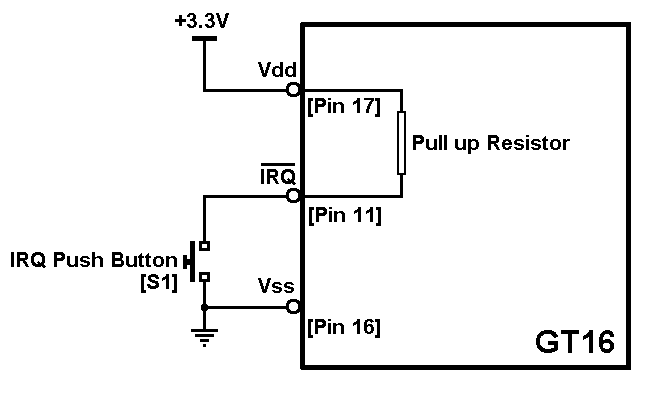
\includegraphics[width=0.7\textwidth]{model.png}
	\caption{Ergodic HMM graphical model showing the hidden states, observation, and transitions between states}
	\label{fig:model}
\end{figure}
%% TODO: Draw a simplified diagram of the 16 connected states with observations

\subsection{Data pre-processing}

\subsection{Parameters of the model}
As a reminder, a continuous HMM model is completely specified by its initial state distribution: \(\pi\) transition matrix: A; the mean covariance matrices: \(\mu\), \(\Sigma\) which can be combined into \(\Phi\). If the observations are modelled with gaussian mixture distributions, an addition parameter is added for the initial mixture distribution: \(\beta\). The next section how each parameters were estimated in this project.

\subsubsection{Transition matrix: A}
For each of the front and back 4-state HMM, the state transition matrix is a 4-by-4 matrix. Two different approaches were considered in the estimation of A. The two methods make use of expectation maximisation algorithm but differ in the modelling of the underlying mechanism.

\begin{enumerate}
	%%TODO draw markov chain diagram
	\item Approach 1: Exploiting available ground truth\\
	This approach takes advantage of the ground truth for a labelled dataset to reduce the HMM model to a Markov Chain. Thus, the hypothetical observation sequence is made identical to the state sequence. Similar to discrete HMM, the transition matrix can be estimated using maximum likelihood algorithms. This approach however makes two assumptions. It not only assumes assumes that the number of states is known but also requires labelled data. Fortunately, the second approach eliminates these constraints. \\\\\
	%%TODO: Quote [1] Durbin, R., S. Eddy, A. Krogh, and G. Mitchison. Biological Sequence Analysis. Cambridge, UK: Cambridge University Press, 1998.
	
	\item Approach 2: This method is the standard approach found in literature using expectation algorithm such as Welch-Baum algorithm. %%TODO: cite 
	%%TODO: site papers to support claim 

\end{enumerate}

\subsubsection{Mean and covariance matrices: \(\mu\) and \(\Sigma\)}

\subsubsection{Inital state distribution}
\begin{enumerate}
	\item Gaussian distribution
	\item Gaussian mixture distribition
	\end{enumerate}
\subsection{Dimension reduction}
\subsubsection{From 18 to 4 features using classification with knn}
\subsection{Continuous observations/features to Discrete observations/features}

\section{HMM implementation}